%%
%% This is file `sample-authordraft.tex',
%% generated with the docstrip utility.
%%
%% The original source files were:
%%
%% samples.dtx  (with options: `authordraft')
%% 
%% IMPORTANT NOTICE:
%% 
%% For the copyright see the source file.
%% 
%% Any modified versions of this file must be renamed
%% with new filenames distinct from sample-authordraft.tex.
%% 
%% For distribution of the original source see the terms
%% for copying and modification in the file samples.dtx.
%% 
%% This generated file may be distributed as long as the
%% original source files, as listed above, are part of the
%% same distribution. (The sources need not necessarily be
%% in the same archive or directory.)
%%
%% The first command in your LaTeX source must be the \documentclass command.
\documentclass[sigconf,authordraft]{acmart}

%%
%% \BibTeX command to typeset BibTeX logo in the docs
\AtBeginDocument{%
  \providecommand\BibTeX{{%
    \normalfont B\kern-0.5em{\scshape i\kern-0.25em b}\kern-0.8em\TeX}}}

%% Rights management information.  This information is sent to you
%% when you complete the rights form.  These commands have SAMPLE
%% values in them; it is your responsibility as an author to replace
%% the commands and values with those provided to you when you
%% complete the rights form.
\setcopyright{acmcopyright}
\copyrightyear{2019}
\acmYear{2019}
\acmDOI{10.1145/1122445.1122456}

%% These commands are for a PROCEEDINGS abstract or paper.
\acmConference[MSWIM '19]{MSWIM '19: The 22nd ACM International Conference on Modeling, Analysis
and Simulation of Wireless and Mobile Systems}{November 25--29, 2019}{Miami, USA}
\acmBooktitle{MSWIM '19: The 22nd ACM International Conference on Modeling, Analysis
and Simulation of Wireless and Mobile Systems,
November 25--29, 2019, Miami, USA}
\acmPrice{15.00}
\acmISBN{978-1-4503-9999-9/18/06}


%%
%% Submission ID.
%% Use this when submitting an article to a sponsored event. You'll
%% receive a unique submission ID from the organizers
%% of the event, and this ID should be used as the parameter to this command.
%%\acmSubmissionID{123-A56-BU3}

%%
%% The majority of ACM publications use numbered citations and
%% references.  The command \citestyle{authoryear} switches to the
%% "author year" style.
%%
%% If you are preparing content for an event
%% sponsored by ACM SIGGRAPH, you must use the "author year" style of
%% citations and references.
%% Uncommenting
%% the next command will enable that style.
%%\citestyle{acmauthoryear}

%%
%% end of the preamble, start of the body of the document source.
\usepackage[utf8]{inputenc}
\begin{document}

%%
%% The "title" command has an optional parameter,
%% allowing the author to define a "short title" to be used in page headers.
\title{Simulation of ISO/IEEE 11073 Personal Health Devices in WBANs}

%%
%% The "author" command and its associated commands are used to define
%% the authors and their affiliations.
%% Of note is the shared affiliation of the first two authors, and the
%% "authornote" and "authornotemark" commands
%% used to denote shared contribution to the research.
\author{Robson A. Lima}
% \authornote{Both authors contributed equally to this research.}
\email{robsonal@midiacom.uff.br}
%\orcid{1234-5678-9012}
\author{Vinicius C. Ferreira}
% \authornotemark[1]
\email{vinicius@midiacom.uff.br}
\author{Egberto Caballero}
% \authornotemark[1]
\email{egbertocr@midiacom.uff.br}
\author{Débora C. Muchaluat Saade}
% \authornotemark[1]
\email{debora@midiacom.uff.br}
\author{Célio V. N. Albuquerque}
% \authornotemark[1]
\email{celio@midiacom.uff.br}
\affiliation{%
  \institution{MídiaCom Lab, Institute of Computing}
  %\streetaddress{}
  \city{Niterói}
  \state{Rio de Janeiro}
  \postcode{24210-240}
}

% \author{Lars Th{\o}rv{\"a}ld}
% \affiliation{%
%   \institution{The Th{\o}rv{\"a}ld Group}
%   \streetaddress{1 Th{\o}rv{\"a}ld Circle}
%   \city{Hekla}
%   \country{Iceland}}
% \email{larst@affiliation.org}

% \author{Valerie B\'eranger}
% \affiliation{%
%   \institution{Inria Paris-Rocquencourt}
%   \city{Rocquencourt}
%   \country{France}
% }

% \author{Aparna Patel}
% \affiliation{%
%  \institution{Rajiv Gandhi University}
%  \streetaddress{Rono-Hills}
%  \city{Doimukh}
%  \state{Arunachal Pradesh}
%  \country{India}}

% \author{Huifen Chan}
% \affiliation{%
%   \institution{Tsinghua University}
%   \streetaddress{30 Shuangqing Rd}
%   \city{Haidian Qu}
%   \state{Beijing Shi}
%   \country{China}}

% \author{Charles Palmer}
% \affiliation{%
%   \institution{Palmer Research Laboratories}
%   \streetaddress{8600 Datapoint Drive}
%   \city{San Antonio}
%   \state{Texas}
%   \postcode{78229}}
% \email{cpalmer@prl.com}

% \author{John Smith}
% \affiliation{\institution{The Th{\o}rv{\"a}ld Group}}
% \email{jsmith@affiliation.org}

% \author{Julius P. Kumquat}
% \affiliation{\institution{The Kumquat Consortium}}
% \email{jpkumquat@consortium.net}

%%
%% By default, the full list of authors will be used in the page
%% headers. Often, this list is too long, and will overlap
%% other information printed in the page headers. This command allows
%% the author to define a more concise list
%% of authors' names for this purpose.
\renewcommand{\shortauthors}{Lima, et al.}

%%
%% The abstract is a short summary of the work to be presented in the
%% article.
\begin{abstract}
Simulating new protocols for e-health systems is very important, as it allows an initial evaluation before a real implementation is made. On the other hand, network simulators do not offer proper support to represent medical applications or components to facilitate running simulations modeling e-health applications. Aiming at fulfilling this gap, this paper proposes a free and open-source implementation of Personal Health Devices (PHD) for Castalia Simulator. We implemented five different PHDs to act like real ISO/IEEE 11073 devices in Wireless Body Area Network (WBAN) simulations. Our implementation supports Agent-initiated mode, where the PHDs take the initiative to send measurements to the hub as also Manager-initiated mode, where the hub require the measurements to PHDs. Our implementation also supports a confirmed communication mode, where the receiver sends an  acknowledgment to the sender every time it receives a packet. Simulation results showed that the confirmed communication mode did not perform well in WBANs when the interval between the transmission are too small, due to the long period of timeout proposed in the ISO/IEEE 11073 standard. Therefore, we propose an extension to the confirmed mode standard that decreases the overhead of control packets over the network and consequently using less timeouts and delivering more packets. 
In contrast, the unconfirmed communication mode, where the sender does not require a confirmation of the packets sent, delivered almost all packets because it had no reliability mechanism that require timeouts.
%This is called confirmed and unconfirmed services type in 11073 standards. We also propose a modification in confirmed serive type.  
\end{abstract}

%%
%% The code below is generated by the tool at http://dl.acm.org/ccs.cfm.
%% Please copy and paste the code instead of the example below.
%%
 \begin{CCSXML}
<ccs2012>
<concept>
<concept_id>10003033.10003039.10003051</concept_id>
<concept_desc>Networks~Application layer protocols</concept_desc>
<concept_significance>500</concept_significance>
</concept>
<concept>
<concept_id>10003033.10003079.10003081</concept_id>
<concept_desc>Networks~Network simulations</concept_desc>
<concept_significance>500</concept_significance>
</concept>
</ccs2012>
\end{CCSXML}

\ccsdesc[500]{Networks~Application layer protocols}
\ccsdesc[500]{Networks~Network simulations}
%%
%% Keywords. The author(s) should pick words that accurately describe
%% the work being presented. Separate the keywords with commas.
\keywords{WBAN, personal health devices, ISO/IEEE 11073, Castalia}

%% A "teaser" image appears between the author and affiliation
%% information and the body of the document, and typically spans the
%% page.
% \begin{teaserfigure}
%   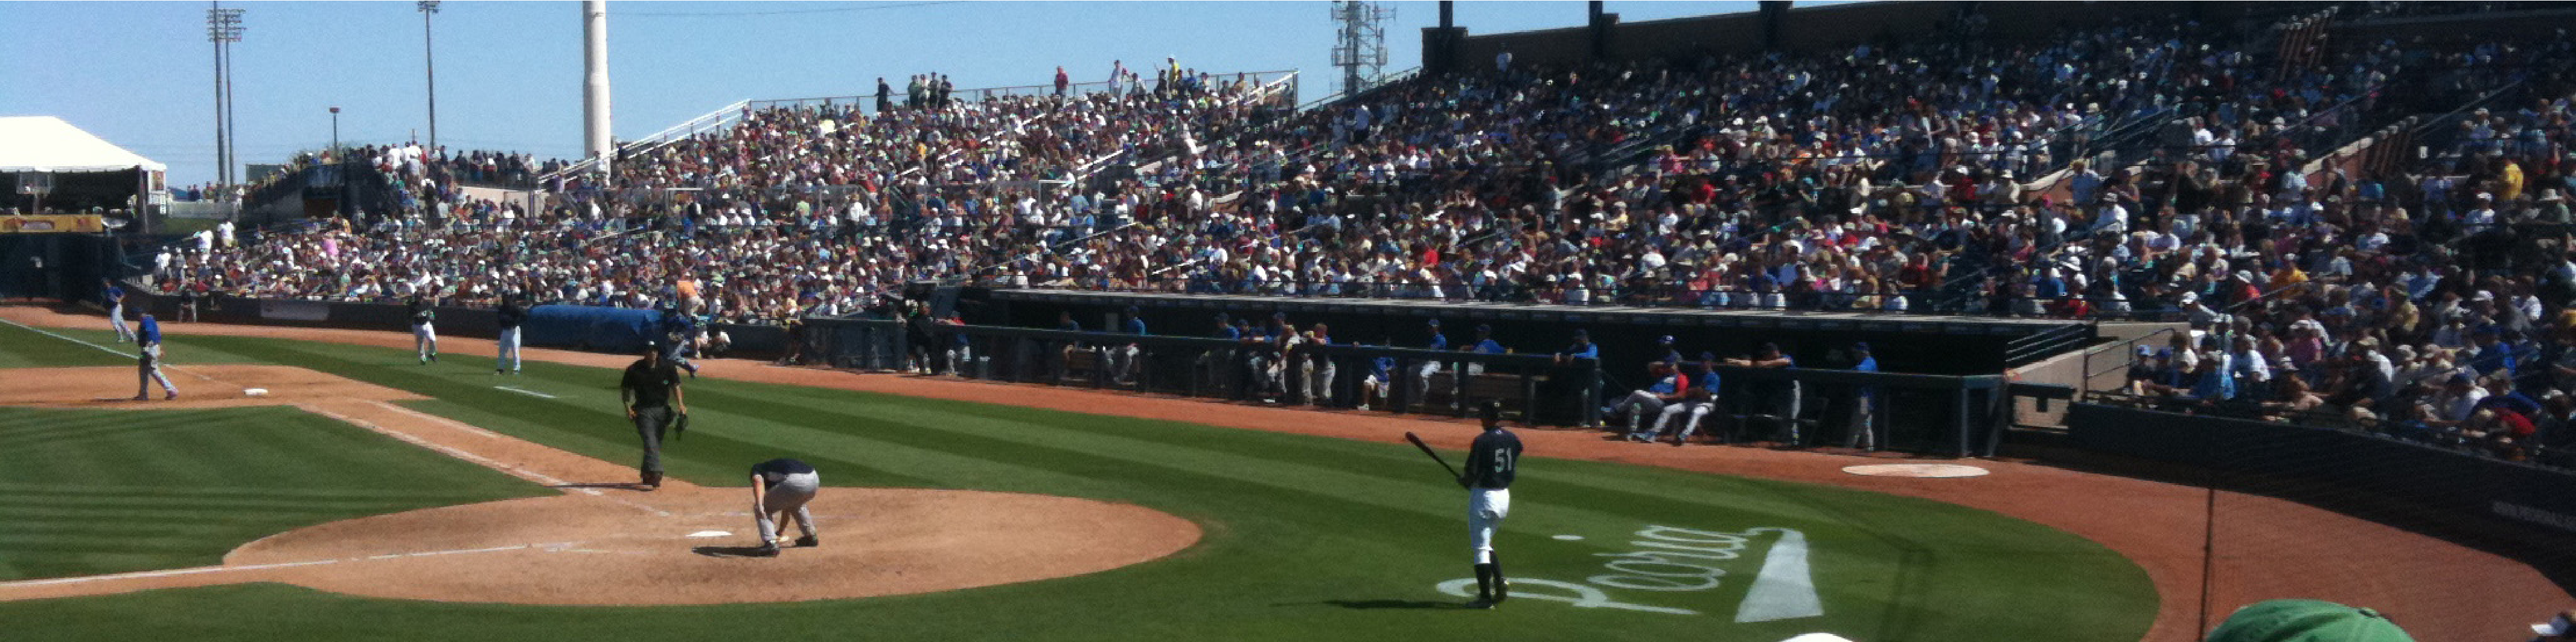
\includegraphics[width=\textwidth]{sampleteaser}
%   \caption{Seattle Mariners at Spring Training, 2010.}
%   \Description{Enjoying the baseball game from the third-base
%   seats. Ichiro Suzuki preparing to bat.}
%   \label{fig:teaser}
% \end{teaserfigure}

%%
%% This command processes the author and affiliation and title
%% information and builds the first part of the formatted document.
\maketitle

\section{Introduction}

Wireless Sensor Networks (WSNs) can be applied to different scenarios, such as Internet of Things, Smart Cities, Medical Systems, etc. Due to increasing research efforts in WSN and telemedicine areas, a new type of network emerged: Wireless Body Area Networks (WBANs) or Body Area Networks (BANs) \cite{b21}. A WBAN consists of intelligent devices, attached to the skin or implanted in the body, capable of exchanging data over a wireless network \cite{b18}.

The lack of commercial devices and health hazards make real experiments with WBANs rare. Therefore, simulation is an important tool to allow feasible tests with less cost and time. Castalia \cite{b15} is a widely used free and open source simulator for wireless sensor networks and wireless body area networks. 

In Castalia, a body sensor is represented by a node that performs network functions, but the applications available in the simulator are generic, and do not specify the type sensor with its communication requirements. 

In order to represent a more realistic simulation scenario, the use of a real standardized medical application is vital. The ISO/IEEE 11073 standard for Personal Health Devices (X73-PHD) describes data exchange, data representation, and terminology for communication between Personal Health Devices. Thus, this standard can be used as a role model for medical applications in our scenario.

The term PHD involves both medical devices and health/fitness devices used in private homes \cite{b3}. The ISO/IEEE 11073 family of standards is divided into three groups, the first and oldest part is the ISO/IEEE 11073 \textit{Lower Layer}, which specifies protocols and communication service using physical layers such as infrared, wireless RF or Ethernet \cite{b16}. The ISO/IEEE 11073 \textit{Point-of-Care-Devices} (X73-PoC) specifies communication standards for devices that are used exclusively in health facilities. Finally, the X73-PHD, sets standards for personal devices used in private homes.
%VINICIUS - O que são "lay" users?, R: eu quis dizer usuários leigos mas já retirei essa palavra%

The X73-PHD standard defines two types of devices: Agents and Managers. Agents are typically low power sensors or actuators, with limited processing power, whereas managers are devices with a greater processing power, that could be connected to an energy source.

The goal of this work is to propose the use of X73-PHD standard in e-health network simulations, representing realistic medical applications and investigating the behavior of medical devices (sensors or actuators) in WBAN scenarios. Examples of personal health devices are oximeters, thermometers, ECGs, glucose meters, blood pressure monitors, etc. 

%This paper proposes a free and open-source implementation of Personal Health Devices for  Castalia  Simulator.  
We  implemented  five  different PHDs   to   act   like   real  X73-PHD   devices   in   WBAN  simulations using the Antidote Library \cite{b20} as a basis.  Our  implementation also   supports   a   confirmed   communication   mode,   where the receiver  sends  an  acknowledgement  to  the  sender  every  time  it receives  a  packet. The 11073 standard was created as an application layer relying on reliable transport layer services. However, in many WSNs and WBAN scenarios, the transport layer is absent. Therefore, the protocol's reliable data transfer mechanism had to be adjusted to the dynamics of a faulty wireless channel, and the lack of transport layer services. Thus, we  propose  an  extension  to  the  standard  that  decreases  the overhead  of  control  packets  over  the  network. 

The rest of the paper is organized as follows: In Section \ref{relatedworks}, we present related works, focusing on X73-PHD works. In Section \ref{systemarch}, an overview of our proposal is given. In Section \ref{castaliaapplayer}, we discuss the parameters available for the user to configure his/her simulation. Results are given in Section \ref{results} and, finally, conclusions in Section \ref{conclusion}.
\section{Related Works}\label{relatedworks}

The Optimized Exchange Protocol (IEEE 11073-20601) is the core of X73-PHD family. It defines the communication syntax in the Domain Information Model (DIM), machine states and services types in the Service Model and procedures in the Communication Model. 

The Domain Information Model defines all common classes and data types used by device types. These classes are expanded by the specialization profiles according to the needs of each device. The Service Model defines the types of messages that can be exchanged between an agent and a manager and the conceptual context in which they are being transmitted \cite{b17}. The communication model defines the procedures to be followed under a normal operation, an exit condition, or when an error occurs.

The 11073 family of standards includes specialization profiles, that is, each agent has an associated standard that describes its data representation. For example, the standard 11073-10408 sets standards for a thermometer, and the 11073-10415 for a balance. These specialization defines the DIM of each device, its attributes, methods, and events of each agent class.

Antidote Stack or Antidote Library is an implementation of the Optimized Exchange Protocol (IEEE 11073-20601) developed by Signove as part of the SigHealth Platform \footnote{SigHealth is a platform for remote patient monitoring and data management using personal wireless devices for health.}. 
%This library is the first open source implementation of this standard, and was developed in ANSI-C with modular architecture, which allows code portability for different platforms. 

%With the popularization of the 11073 standard, several improvements were proposed to enhance the operation and interoperability. 
In \cite{b7},\cite{b8} and \cite{b9} the integration of X73-PHD and IoT protocols, such as MQTT and COaP, are proposed to be used as transport protocols, enabling personal health devices to share health information directly through the Internet, using low power consumption and few control messages. Those works also discuss the availability of enabling IoT technologies for health information as well as the mapping of messages from X73-PHD into IoT protocols. All those works used real devices with Antidote as their application layer protocol.

Another project on 11073 standards is \cite{b11}, which has developed an interoperable end-to-end remote patient monitoring platform using ZigBee Health Care Profile as transport layer and a Machine to Machine (M2M) solution to provide wide area network connectivity. That work also includes a web application on the clinical side (server side) and use the standards and frameworks provided by Integrating the Healthcare Enterprise (IHE) \cite{b13} and Health Level Seven (HL7) \cite{b12} to ensure end-to-end interoperability. Those two companies advocate a world in which everyone can securely access and use the right health data when and where they need it.

The X73-PoC version provides a mechanism to remotely control agents. This mechanism is defined in the standards X73-10201 and X73-20301. However, the X73-PHD has no mechanisms to do such a thing. So, in \cite{b14} the author proposes to adapt the remote control capabilities from X73-PoC to X73-PHD with an acceptable overhead and no extra cost to manufacturers. This mechanism has to be installed in manager and agents, and the remote control consists of being able to change the units of measurements (e.g. - changing from kilograms to pounds) directly from the manager, a smartphone or a computer engine in nursing units.

In this work, we use the Antidote library to run the agent and manager X73-PHD stack over Castalia. Five different device profiles are used: 11073-10406 Basic electrocardiograph (1 to 3 lead ECG), 11073-10404 Pulse oximeter, 11073-10408 Thermometer, 11073-10417 Glucose meter, and 11073-10407 Blood pressure monitor. All these agents are used to represent body sensors in WBAN simulations. To fulfill that purpose, the X73-PHD reliable data transfer mechanism was adjusted to work on a WBAN scenario, a wireless environment, with a faulty media, and lacking transport layer services.

%VINICIUS - Eu tirei pra deixar o capítulo todo mais focado em PHD%
%In \cite{b6} the authors presents an open-source energy-harvesting simulation framework called GreenCastalia which supports multi-source and multi-storage energy harvesting architectures developed for the Castalia simulator. GreenCastalia project focus is to simulate realistic battery discharge on devices. The majors modifications to the original Castalia code was made to the Resource Manager module. Also in this module the authors adds the energy-harvesting systems that provides a more realistic battery model.
\section{System Architecture}\label{systemarch}

Antidote has a plug-in based architecture. So, a Castalia plugin was developed to support communication between Antidote Stack and Castalia Modules. As the Antidote is developed to work with real devices, modifications had to be made to the library to work in Castalia Simulator. The communication, encoders, agent and manager are some of the Antidote's modules modified.

\subsection{Castalia Plugin}

Antidote itself is portable and uses ANSI C language to create a standard and clean library. To provide a communication between Antidote and other systems, like Castalia, we must adapt and develop the necessary communication plug-ins.

The proposed plug-in allows Castalia and Antidote to talk with each other through Castalia plug-in module. Inside Castalia, we can call any function from Antidote Library and retrieve any information from it, but transmitting data from Castalia to Antidote Library is not a simple task. To solve this, we first use external variables to make the data exchange between Castalia and Castalia plug-in module. Then, to obtain the data from Castalia plug-in module, Antidote uses pointers to Castalia plug-in functions that we call \textit{callback functions}. That is why we need a plug-in to mediate the communication. 

There is a set of callback functions in Castalia plug-in module that are passed to Antidote during the initialization process of each agent. These callback functions are passed to communication module of Antidote as pointers to functions. This way, whenever the communication module needs to retrieve or send a message, it just triggers the correspondent callback function. 
%The task of these callback functions is to receive and send messages as also initialize and finalize a agent network.

Figure~\ref{fig:CastaliaPlugin} depicts how Antidote gets messages from Castalia. The arriving messages are copied to an external variable in Castalia Simulator Module - the external variable is visible to both Castalia Simulator and Castalia Plugin module. Since the communication module in Antidote owns pointers to Castalia Plug-ins functions, it can retrieve the messages using callback functions.

\begin{figure}[htbp]
\centerline{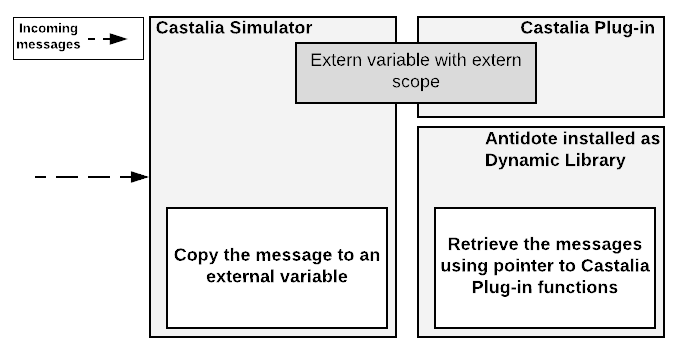
\includegraphics[scale=0.35]{figures/castaliaPlugin.png}}
\caption{How Antidote Library gets messages from Castalia Simulator.}
\label{fig:CastaliaPlugin}
\end{figure}

\subsection{Changes in communication module}

The Communication module is one of the most important modules in the Antidote Library. The start, the end, transmissions, machine state phases of all nodes are controlled by this module. In a real scenario, each device has its own communication module, running its own copy of the code. But in a single-machine simulation, it is a bit different. Only one communication module has to handle all nodes, since the Antidote Library is installed in the operating system as a dynamic library.

To ensure the proper operation of the Communication Module, the \textit{node id} is required in each function call, this way we know which node we are working with and apply the action for that node, without affecting other nodes. For example, if a node transits from unassociated state to associating machine state, without the proposed modification, this action would affect all nodes even those that should not change their machine states.

Figure~\ref{fig:communicationModuleCastalia} illustrates the system modification. In every function in the Communication module, we insert the \textit{node id} new parameter. This way the communication module always knows the corresponding node. 
%The arrows in Fig.~\ref{fig:communicationModuleCastalia} represents functions calls.

\begin{figure}[htbp]
\centerline{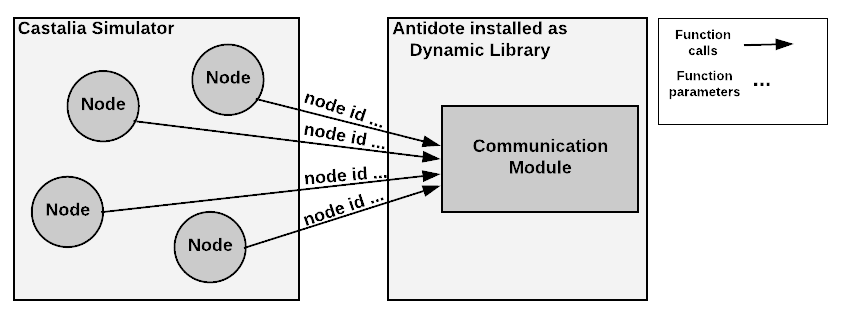
\includegraphics[scale=0.31]{figures/communicationModule.png}}
\caption{Communication module handling several nodes. Each arrow represents a function being called from the Communication Module.}
\label{fig:communicationModuleCastalia}
\end{figure}

\subsection{Other modifications}

Other modules like Agent, Manager and Encoders were modified to smooth operation of Antidote functions in Castalia. We can highlight the function created in the encoder module to convert absolute values (the measurements) into scaled non-negative values as recommended by \cite{b1}.
%Functions to finalize the Agents module were transferred to Manager module for the sake of simplicity and the \textit{node id} were add as a parameters of Agent and Manager functions.
%In Encoder module a function to interpret the data received was created.
It is useful to send absolute values like $-0.060$  which would require at least 4 bytes in X73-PHD floating point format. When converted, the number $-0.060$ becomes $388$, which requires just two bytes. The X73-PHD standard defines its own floating point types composed of a 32-bit word comprising a signed 8-bit integer exponent followed by a signed 24-bit integer mantissa.
%VINICIUS - acho melhor especificar pq falar só "many" fica muito genérico. R: feito.

Within the Manager, the equation to make the conversion from scaled to absolute values is given by expression\\$Y = M \times X + B$, where:
\begin{align*}
    Y &= \text{the converted absolute value}\\
    M &= \frac{(\text{upper absolute value} - \text{lower absolute value})}{(\text{upper scaled value} - \text{lower scaled value})}\\
    B &= \text{upper absolute value} - (M \times \text{upper scaled value})\\
    X &= \text{the scaled value}
\end{align*}

Within an Agent, the conversion from absolute values to scaled values is given by expression $X = \frac{(R - B)}{M}$, where: $R =$ actual measured value.

%\begin{align*}
%    R &= \text{actual measured value}
%\end{align*}

A thermometer that does readings from $-45^\circ$C  to $50^\circ$C with a resolution of $0.5^\circ$C has the following values: lower absolute value = $-45.0$, upper absolute value = $50.0$, lower scaled value = $0$, upper scaled value = $190$. Giving $M = 0.5$ and $B = -45.0$.

%\begin{align*}
%    \text{Lower absolute value} &= -45.0 \\
%    \text{Upper absolute value} &= 50.0 \\
%    \text{Lower scaled value} &= 0 \\
%    \text{Upper scaled value} &= 190
%\end{align*}

%Giving $M = \frac{(50.0 - (-45.0))}{(190 – 0)} = 0.5$ and $B = 50.0 - (0.5 \times 190) = -45.0$

The Castalia plug-in module and the modifications to Antidote Library were made exclusively for WBAN simulation in Castalia.

%VINICIUS - talvez uma conclusão dessa seção fosse inteiressante, R: Feito
\section{Castalia Application Layer}\label{castaliaapplayer}

We have created an application for the Castalia Application Layer. This application is agent and manager-initiated, that is, the agent takes the initiative to send readings to the manager or the manager may request measurements to an agent. The agent is the first and the only one to send an \textit{Association request} to start sending measurements. To stop a transmission in agent-initiated mode, agents can send an \textit{Association Release} message when there is no more measurements to be sent. In the manager-initiated mode a \textit{Stop Request} message is send to an agent requesting the stop measurement data transmission.

The proposed application has five agent types: pulse oximeter, glucose meter, thermometer, blood pressure monitor and a basic ECG. The pulse oximeter transmits the pulse rate in beats per second and the percentage of arterial hemoglobin oxygen saturation (SpO$_2$). The glucose meter sends the glucose level, that is, the concentration of glucose in the blood in milligrams per deciliter (mg\//dL). The thermometer measures temperature in Celsius (\textdegree C). The blood pressure sends a data compound of systolic, diastolic and the mean arterial pressure in millimeters of mercury (mmHg). The basic ECG sends eighty samples of the heart's electric potential in millivolt (mV) per packet. Each mV sample has to be converted to scaled non-negatives values before sent. 
%The lower and upper absolute values and the lower and upper scaled values are transmitted in the configuration phase. 
All these agents samples are randomly produced, except the basic ECG that transmits real values obtained from the data base \cite{b2}.

The X73-PHD standard defines \textbf{confirmed} and  \textbf{unconfirmed events}. The confirmed events expect a reception acknowledgment from the manager and the unconfirmed events do not. Control messages, like \textit{Association request} and \textit{Association release}, are always sent in confirmed mode, but measurements can be configured to use confirmed or unconfirmed mode.
The standard also defines three modes of manager-initiated measurement data transmission: \textbf{Single Response}, \textbf{Time Period} and \textbf{No Time Limit Mode}. The Single Response Mode allows the manager to explicitly request a single data from the agent and receive it in the response message.  The Time Period Mode is used by the manager to enable an agent to send any data it collects for the duration of the requested time period. The No Time Limit Mode shall be used to order an agent to send event reports continually until a \textit{Stop Request} message is received or the association between the agent and the manager is terminated.
%The implemented parameter to set the desired mode is \textit{SN.node\[node number\].Application.confirmed\_event} which require a Boolean value.

In our application, the user can set some simulation's parameters like: the medical device type, thermometer, pulse oximeter, blood pressure and etc, the transmission rate in measurements per seconds, the events types confirmed/unconfirmed and the manager-initiated mode data transmission. If no manager-initiated mode is set, the application uses Agent-initiated mode.

\subsection{Unconfirmed measurement event}\label{sec:UnconfirmedMeasurementEvent}

Figure~\ref{fig:unconfirmedMode} shows a sequence diagram of the messaging process corresponding to an ordinary operation of an agent with standard configuration and with unconfirmed measurement events. The agent intends to associate with the manager for the first time, and sends an \textit{Association request}. When the manager receives the \textit{Association request}, it checks if the agent was previously associated. If it is the agent's first association, the manager sends a \textit{Get attributes} message along with the \textit{Association response}. So, the agent sends its configuration and starts to send the measurements to the manager. When there are no more readings to transmit, the agent sends an \textit{Association release} and the manager responds with an \textit{Association release response}.

\begin{figure}[htbp]
\centerline{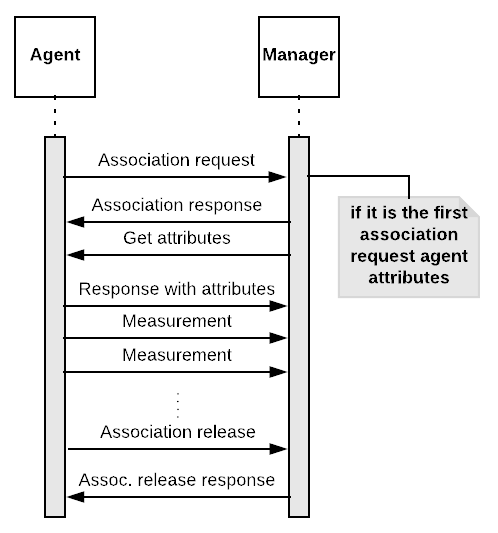
\includegraphics[scale=0.35]{figures/unconfirmed.png}}
\caption{Sequence diagram of unconfirmed operation mode of an 11073 PHD application.}
\label{fig:unconfirmedMode}
\end{figure}

\subsection{Confirmed measurement event}

Figure~\ref{fig:confirmedMode} depicts a sequence diagram of the messaging procedure corresponding to an operation of an agent with standard configuration and with confirmed measurements events. The initial procedure is the same as explained in Section \ref{sec:UnconfirmedMeasurementEvent}, the difference is that the manager sends an acknowledgment for every measurement received. After sending a measurement data, the agent must wait three seconds for an ACK. If an ACK is not received in this period, the agent sends an \textit{Association abort} to the manager, and transits to the unassociated state. If the agent still has readings to send, a new association must be made.

\begin{figure}[htbp]
\centerline{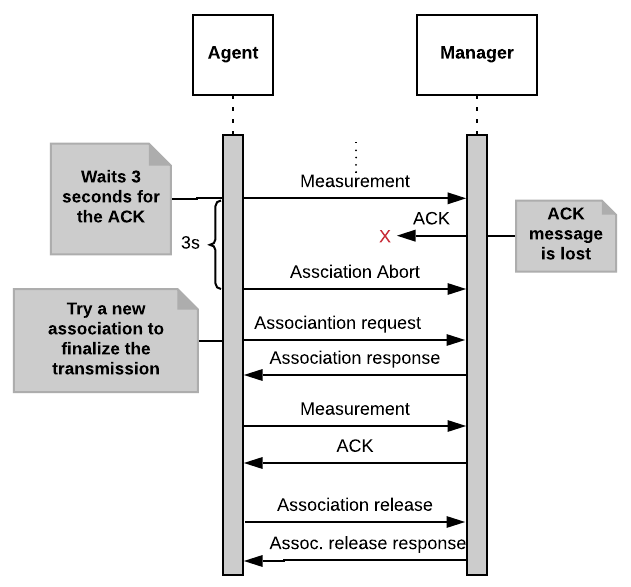
\includegraphics[width=\linewidth]{figures/confirmedModeWithAckLoss.png}}
\caption{Sequence diagram of confirmed operation mode of an 11073 PHD application.}
\label{fig:confirmedMode}
\end{figure}

\subsection{Proposed modification in confirmed measurement events}

The X73-PHD standard assumes that there will be a reliable transport layer on real devices. In the Castalia simulator, as in usual wireless sensor networks, a transport layer could not be used. So we propose a stop-and-wait system as a sub-application-layer to retransmit agent packets whose ACK have not been received.
%To avoid many associations right after a non-received ACK we implemented a stop-and-wait retransmission system in the application layer. 
It reduces the unnecessary exchange of several control packets made in association procedures. Rather than making a new association when an ACK is lost, we just retransmit the packet $n$ times or until an ACK is received.
%The user can define whether to retransmit and how many retransmission attempts wish.
The user may define a number $n$ of retransmissions, and the agent will retransmit that message up to $n$ times until a corresponding ACK is received. If the manager receives a duplicated message, it will retransmit immediately another ACK to the agent. We call it \textbf{Retransmission Mode}.

In Section \ref{results}, we evaluate this solution's efficiency in reducing control packets exchange in a WBAN scenario. Note that this is a new proposal, not present in the X73-PHD standard. In Figure~\ref{fig:retransmissionMode}, is shown a sequence diagram for a data measurement transmission using retransmission mode. In this figure two case are addressed: An ACK for a data measurement is not received and a data measurement is lost.
%The parameters implemented for retransmission are \textit{SN.node[nodeNumber].Application.retransmissionPacket} which require a boolean value and \textit{SN.node[nodeNumber].Application.maxNumOfRetransmition} that accepts an integer number.

\begin{figure}[htbp]
\centerline{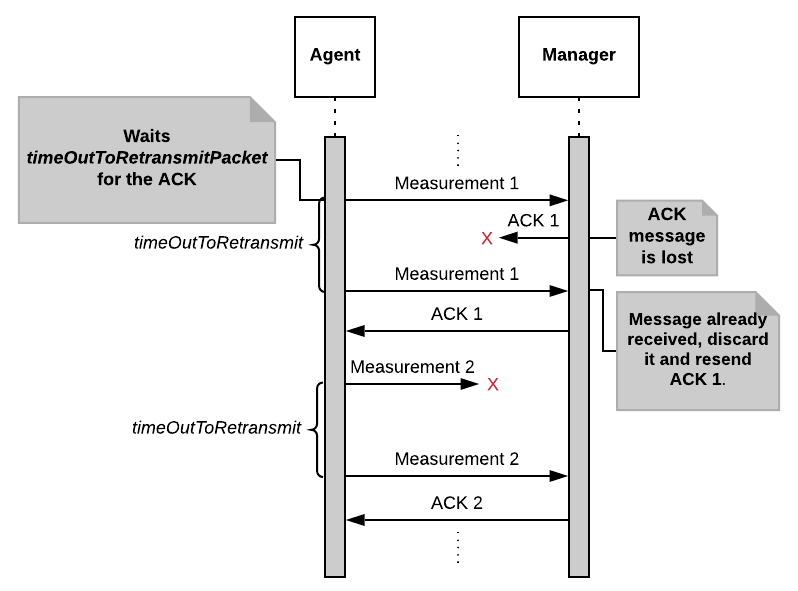
\includegraphics[width=\linewidth]{figures/retransmissionModeWithAckLoss.png}}
\caption{Sequence diagram of retransmission operation mode of an 11073 PHD application.}
\label{fig:retransmissionMode}
\end{figure}

\subsection{Manager-initiated modes}

Figure~\ref{fig:managerinitiated} depicts a sequence diagram of the messaging procedure corresponding to an operation of an agent using manager-initiated events. The initial procedure is the same as explained in above sections. The difference is the \textit{Data Request} control packet. This packet can request measurement data to agents in three ways: Single, Time Period and No Time Period mode. The time has to be defined in Time Period mode.

\begin{figure}[htbp]
\centerline{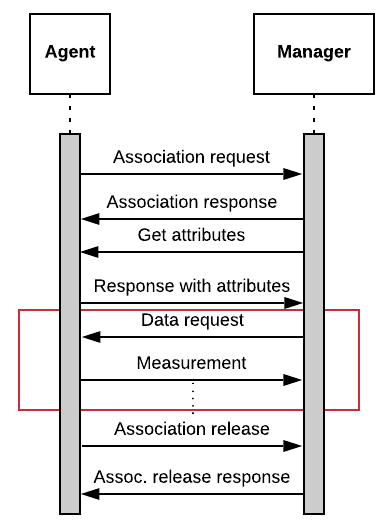
\includegraphics[scale=0.35]{figures/Manager-initiatedmode.png}}
\caption{Sequence diagram of manager-initiated operation mode of an 11073 PHD application}
\label{fig:managerinitiated}
\end{figure}
\section{Use case and simulation parameters}\label{simulationparameter}
All results presented in this section are relative to the application layer. We run simulations on a computer with 8GB RAM memory, CPU Intel Core i5-7200U and Ubuntu 18.04 LTS operating system. All runs lasts 43201s seconds (12 hours) with the first second used just for network setup (e.g., nodes requesting connections). The simulation was executed 15 times with $95\%$ of confidence interval.
%Using some \textit{api} from Castalia Simulator some results like the total number of control packets exchanged, the total number of measurements packets, how many times a packets was retransmited among many others results can be obtained easily.
%\subsection{Use case and simulation parameters}

Remote Monitoring and Independent living for elderly care is one of the use cases of the X73-PHD standard. The sensors and actuators proposed for this use case are: blood pressure monitor, thermometer, glucose meter, pulse oximeter and basic ECG  \cite{b3}. In this work, we have used an hypothetical elderly patient who has cardiac problems, diabetes and hypertension, and needs to be monitored in his home.

Figure~\ref{fig:wbantopology} shows the topology setup used in our simulation. The hub node is placed at the right hip, a sensor node at each wrist, one sensor node at the each ankle, and one sensor on the chest. We used this set to test our proposed features. These nodes' positions have the advantage of experimental measurements of path loss, made for every pair of nodes, as discussed in \cite{b4}.

\begin{figure}[htbp]
\centerline{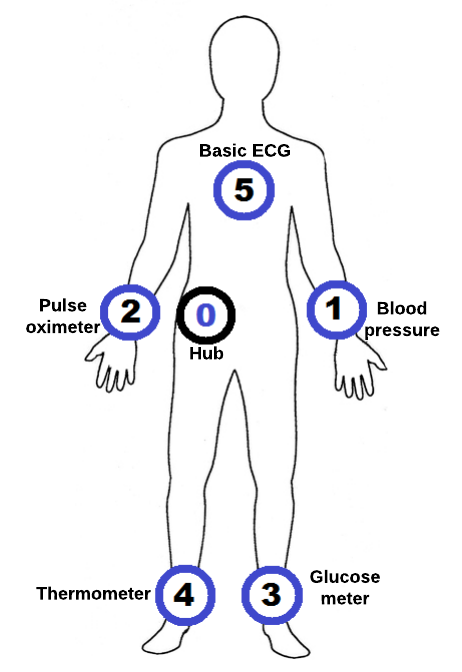
\includegraphics[scale=0.29]{figures/corpoSensoresNomes.png}}
\caption{The simulated network topology.}
\label{fig:wbantopology}
\end{figure}

In this work we simulate six scenarios, three agent-initiated and three manager-initiated.

The first three agent-initiated scenario are: a) Unconfirmed Mode, where the agents takes the initiative to send measurements to the manager without confirmation. b) Confirmed Mode, agents wait for three seconds the ACK from the manager. If an ACK is not received, the agent has to try to establish a new association to finalize the transmission of the measurement packets. c) Retransmission Mode, agents expect an ACK from the manager during the time period defined by the user in \textit{timeOutToRetransmitPacke} and in case it is not received, the packet is retransmitted up to \textit{maxNumOfRetransmition} also define by the user. If all the retries is used and an confirmation is not received, a new association is made. 

The last three manager-initiated scenarios are: a) Single Mode, the manager request just one measurement data to an agent. b) Time Period mode, allows manager to request agents to send measurements data during a time period. c) and finally, the No Time Period Mode where manager request measurements data to the agents continually until the association is break or the manager sends a \textit{Stop Request} message.
%Table \ref{3modes} summarizes the three mentioned modes. 

The MAC layer used is the IEEE 802.15.6 (WBAN) \cite{b5} with path loss map and temporal model for wireless channel supplied by Castalia. The radio used meets with the IEEE 802.15.6 radio proposal \cite{b5} with $-15$dBm as transmission power.
% \begin{table}[htbp]
% \caption{Operational modes supported by the proposed implementation}
% \begin{center}
% \begin{tabular}{lllll}
% \cline{2-4}
%  & \multicolumn{1}{c}{\textbf{\begin{tabular}[c]{@{}c@{}}Unconfirmed\\ mode\end{tabular}}}                      & \multicolumn{1}{c}{\textbf{\begin{tabular}[c]{@{}c@{}}Retransmission\\ mode\end{tabular}}}                                      & \multicolumn{1}{c}{\textbf{\begin{tabular}[c]{@{}c@{}}Confirmed\\ mode\end{tabular}}}                                         &  \\ \cline{2-4}
%  & \begin{tabular}[c]{@{}l@{}}The measurements \\ are transmitted\\ with no ACK from\\ the manager\end{tabular} & \begin{tabular}[c]{@{}l@{}}The measurements \\ are retransmitted\\ if an ACK is not\\ received from the\\  manager\end{tabular} & \begin{tabular}[c]{@{}l@{}}If an ACK is not\\ received, try a\\ new association\\ to continue the \\ transmission\end{tabular} &  \\ \cline{2-4}
% \end{tabular}
% \label{3modes}
% \end{center}
% \end{table}

The configuration of the nodes is set as follows: the total simulation time is $43200$ seconds (12 hours). Node 0 uses the \textit{Manager} application and is the hub. The blood pressure monitor transmits one measurement every $15$ minutes, totalizing $48$ measurements to be sent in our simulation. The thermometer sends one read every $3$ minutes, then, $240$ measurements should be sent. The glucose meter transmits one measurement every $5$ minutes, that is, $144$ measurements in  $43200$ seconds. Thermometer sends the temperature every $3$ minutes then $240$ in total. In this work, we assume the basic ECG as a device that receives signals of all electrodes deployed in the body, and transmit these signals to the manager. So, it will transmit $80$ millivolt samples per $0.8$ seconds, which gives $54000$ measurement packets in $43200$s of simulation.

In the three agent-initiated modes the nodes will try to transmit all the packets described in the paragraph above, but in manager-initiated modes it is not true. The Single Mode for example, transmit just one measurement data packet. For the Time Period Mode we define $21600$ seconds ($6$ hours) of measurement data packets transmission, which is half of the total measurements transmitted in agent-initiated modes. And for the No Time Period mode the manager sends a \textit{Stop Request} message when $10$ measurement data packet is received from every node.     

\section{Results}\label{results}

%All the results that will be presented is already implemented in the proposed application and everyone can feel free to customize it. 
%The results available in the application are the total control packets exchanged per node, the measurements packets received by the manager per node, the measurements packets sent by each node, and the total of associations made per agent. 

The first result discussed is the total of successfully measurements delivered to the manager using the agent-initiated mode.
%As described in \cite{b1}, when an agent is working on confirmed mode, it  should send a measurement packet and wait for the ACK during three seconds.
We can see in Figure~\ref{fig:measurementsDeliveredAgentInitiated} the delivered packets from ECG using confirmed mode is too small. This shows the lack of adaptation of the confirmed mode when the interval to transmit the measurements packet is smaller than the timeouts proposed by the standard. In this case, the bad link quality and consequently the loss of ACKs, use of timeouts for disassociation/reassociation processes took most of the time for measurement transmission. For example, in our simulation the ECG sends one measurements every 0.8s, a timeout for the association process in confirmed mode takes 10s, that is, 12.5 packets that could be transmitted in this timeout period.
The retransmission mode improved the results by reducing the wait time of an association handshake, and retransmitting the messages sooner. The unconfirmed mode delivered almost all packets, although it provides no reliability.
In contrast to the ECG, the thermometer in confirmed mode, Figure~\ref{fig:measurementsDeliveredAgentInitiated}, delivered more than 100\% of the measurement packets because duplicate measurements are taken into account for this result.

\begin{figure}[htbp]
\centerline{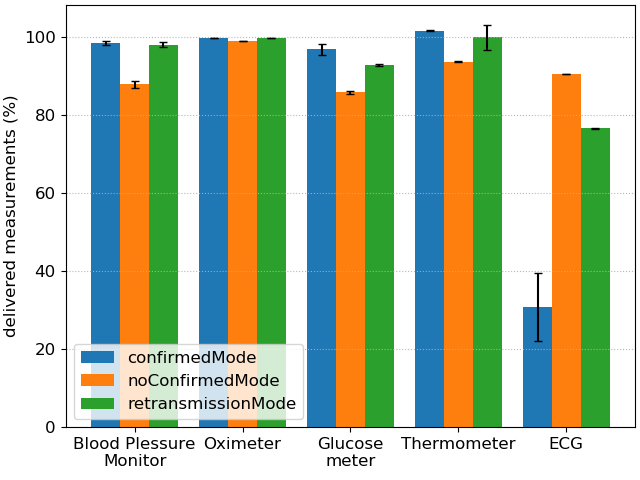
\includegraphics[width=\linewidth]{figures/MeasurementsDelivered-AgentinitiatedMode.png}}
\caption{Measurement packets successfully delivered per node using Agent-initiated mode}
\label{fig:measurementsDeliveredAgentInitiated}
\end{figure}

The delivered measurements packets for the manager-initiated mode can be seen in the Figure~\ref{fig:measurementsDeliveredManagerInitiated}.

\begin{figure}[htbp]
\centerline{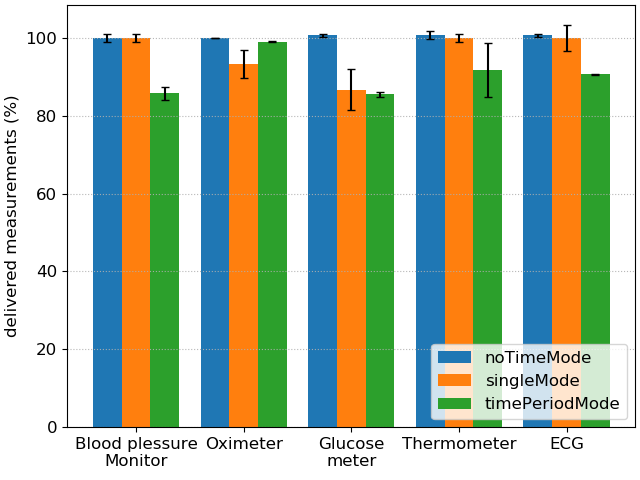
\includegraphics[width=\linewidth]{figures/MeasurementsDelivered-ManagerinitiatedMode.png}}
\caption{Measurement packets successfully delivered per node using Manager-initiated mode}
\label{fig:measurementsDeliveredManagerInitiated}
\end{figure}

The overhead of control packets exchanged between a node and the manager is crucial in this scenario, as in the case of a new association due to a non-received ACK. The association procedure involves a maximum of four packets for a new node, and a minimum of two packets, when the agent's attributes are previously known.

The total of control packets exchanged between each node and the manager per operation mode is depicted in Figure~\ref{fig:controlpacketsexchanged}.
Notice that nodes transmit different number of packets in the same simulation. While the blood pressure monitor convey $48$ measurements in $12$ hours, the ECG has to transmit $54000$ measurements in the same time period. Is expected to save more control packets in retransmission mode when compared to confirmed mode. Although, the ECG in Figure~\ref{fig:controlpacketsexchanged}, the retransmission mode has used more control packets than the confirmed mode due to the first one delivered more measurements packets than the former mode as was seen in Figure~\ref{fig:measurementsDeliveredAgentInitiated}.
%Notice that our retransmission mode saves about $21.5\%$ of control packets when compared to the confirmed mode. 
The unconfirmed mode as expected is the one that transmits less control packets.

\begin{figure}[htbp]
\centerline{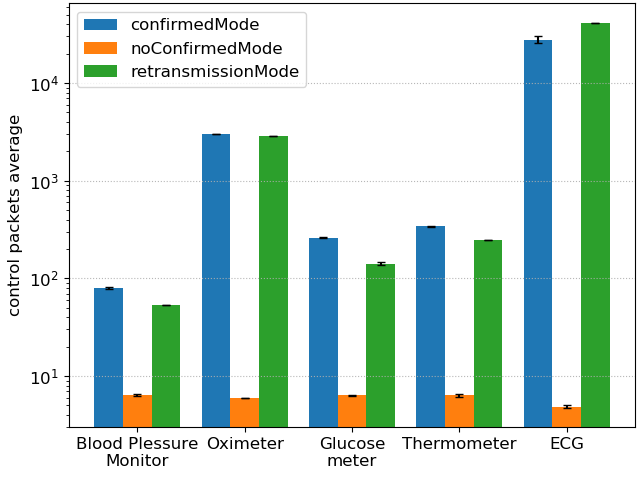
\includegraphics[width=\linewidth]{figures/ControlPacketsPerNode.png}}
\caption{The average control packets exchanged of all nodes in Agent-initiated mode.}
\label{fig:controlpacketsexchanged}
\end{figure}

The number of associations made per node is extremely high with the confirmed mode, since it tries a new association after every packet lost. Figure~\ref{fig:associationnumber} shows the average number of associations that each node made in Agent-initiated modes. As expected, the confirmed mode has the highest average of association attempts, while the unconfirmed mode made just one association. The retransmission mode tries a new association after all the attempts to resend a message, or if the agent receives an abort message from the manager. This is the reason for the low average of associations in this mode. The ECG which has the worst wireless link require almost $2000$ new associations to finalize the transmission of $54000$ measurements in confirmed mode.

\begin{figure}[htbp]
\centerline{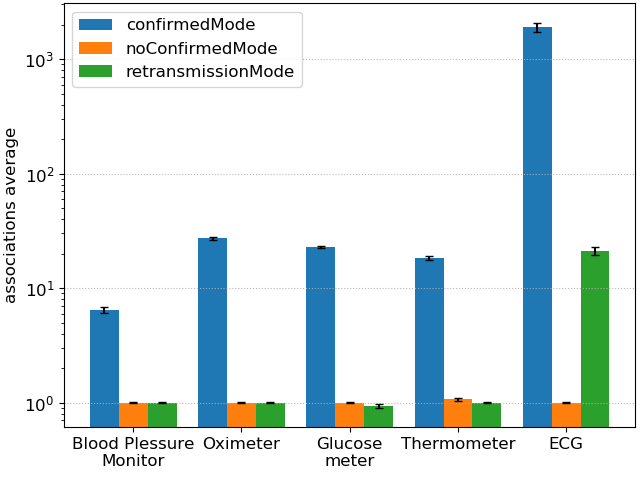
\includegraphics[width=\linewidth]{figures/AssociationsMadePerNode.png}}
\caption{The average numbers of association made per node}
\label{fig:associationnumber}
\end{figure}

In the Figure~\ref{fig:retransmissionretries} we can see the average number of retransmission retries made in the retransmission mode by the application layer. Most packets are successfully delivered in the first try and more than $1000$ packets uses $1$ retransmission retry. In the seventh retransmission retry the values tend to zero.

\begin{figure}[htbp]
\centerline{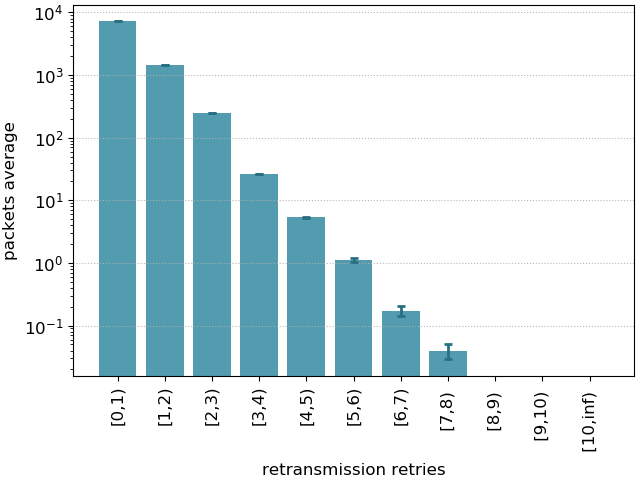
\includegraphics[width=\linewidth]{figures/RetransmissionRetries.png}}
\caption{The average number of packets retransmission made at the application layer}
\label{fig:retransmissionretries}
\end{figure}

The Figure~\ref{fig:latency} shows that most packages have an average latency of $180$ms in retransmission mode and confirmed mode and $30$ms in no confirmed mode. 
The time is calculated from the moment of creation of the package, at the application layer of the agent, until it is received at the application layer of the manager.

\begin{figure*}[htbp]
\centerline{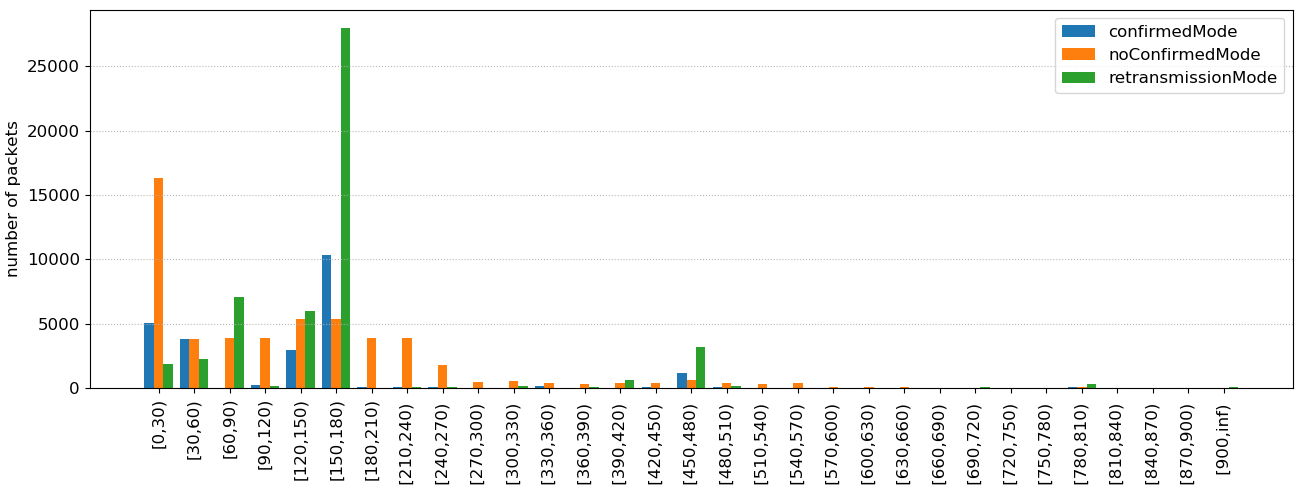
\includegraphics[width=\linewidth]{figures/Latency.png}}
\caption{The latency level in application layer}
\label{fig:latency}
\end{figure*}
\section{Conclusion}\label{conclusion}
In this paper, we have presented a proposal to simulate personal health devices in Castalia Simulator. Our application layer follows the X73-PHD standard with the aid of the Antidote Library. Five agents were implemented, and they simulate real personal health devices. In addition, a new reliable data transfer mode was proposed, the retransmission mode, to adjust the X73-PHD protocol to WBAN scenarios, where a reliable transport layer is usually not available. The retransmission mode aimed at reducing the number of disassociation/reassociations that take place after a message or acknowledgement is lost.

As future work, we intend to calculate the \textit{timeOutToRetransmitPacket} dynamically based on the current latency of a packet. Thus, the user does not need to set this values in the simulation file. The codes for Castalia Application and for Antidote Modified Library can be found respectively at \url{https://github.com/conqlima/Antidote} and \url{https://github.com/conqlima/11073PhdApplication}.
%The results shows the advantages of using the retransmission mode over the standards' confirmed mode, increasing the message delivery ratio and reducing the overhead of the protocol. 


% \section{Introduction}
% ACM's consolidated article template, introduced in 2017, provides a
% consistent \LaTeX\ style for use across ACM publications, and
% incorporates accessibility and metadata-extraction functionality
% necessary for future Digital Library endeavors. Numerous ACM and
% SIG-specific \LaTeX\ templates have been examined, and their unique
% features incorporated into this single new template.

% If you are new to publishing with ACM, this document is a valuable
% guide to the process of preparing your work for publication. If you
% have published with ACM before, this document provides insight and
% instruction into more recent changes to the article template.

% The ``\verb|acmart|'' document class can be used to prepare articles
% for any ACM publication --- conference or journal, and for any stage
% of publication, from review to final ``camera-ready'' copy, to the
% author's own version, with {\itshape very} few changes to the source.

% \section{Template Overview}
% As noted in the introduction, the ``\verb|acmart|'' document class can
% be used to prepare many different kinds of documentation --- a
% double-blind initial submission of a full-length technical paper, a
% two-page SIGGRAPH Emerging Technologies abstract, a ``camera-ready''
% journal article, a SIGCHI Extended Abstract, and more --- all by
% selecting the appropriate {\itshape template style} and {\itshape
%   template parameters}.

% This document will explain the major features of the document
% class. For further information, the {\itshape \LaTeX\ User's Guide} is
% available from
% \url{https://www.acm.org/publications/proceedings-template}.

% \subsection{Template Styles}

% The primary parameter given to the ``\verb|acmart|'' document class is
% the {\itshape template style} which corresponds to the kind of publication
% or SIG publishing the work. This parameter is enclosed in square
% brackets and is a part of the {\verb|documentclass|} command:
% \begin{verbatim}
%   \documentclass[STYLE]{acmart}
% \end{verbatim}

% Journals use one of three template styles. All but three ACM journals
% use the {\verb|acmsmall|} template style:
% \begin{itemize}
% \item {\verb|acmsmall|}: The default journal template style.
% \item {\verb|acmlarge|}: Used by JOCCH and TAP.
% \item {\verb|acmtog|}: Used by TOG.
% \end{itemize}

% The majority of conference proceedings documentation will use the {\verb|acmconf|} template style.
% \begin{itemize}
% \item {\verb|acmconf|}: The default proceedings template style.
% \item{\verb|sigchi|}: Used for SIGCHI conference articles.
% \item{\verb|sigchi-a|}: Used for SIGCHI ``Extended Abstract'' articles.
% \item{\verb|sigplan|}: Used for SIGPLAN conference articles.
% \end{itemize}

% \subsection{Template Parameters}

% In addition to specifying the {\itshape template style} to be used in
% formatting your work, there are a number of {\itshape template parameters}
% which modify some part of the applied template style. A complete list
% of these parameters can be found in the {\itshape \LaTeX\ User's Guide.}

% Frequently-used parameters, or combinations of parameters, include:
% \begin{itemize}
% \item {\verb|anonymous,review|}: Suitable for a ``double-blind''
%   conference submission. Anonymizes the work and includes line
%   numbers. Use with the \verb|\acmSubmissionID| command to print the
%   submission's unique ID on each page of the work.
% \item{\verb|authorversion|}: Produces a version of the work suitable
%   for posting by the author.
% \item{\verb|screen|}: Produces colored hyperlinks.
% \end{itemize}

% This document uses the following string as the first command in the
% source file:
% \begin{verbatim}
% \documentclass[sigconf,authordraft]{acmart}
% \end{verbatim}

% \section{Modifications}

% Modifying the template --- including but not limited to: adjusting
% margins, typeface sizes, line spacing, paragraph and list definitions,
% and the use of the \verb|\vspace| command to manually adjust the
% vertical spacing between elements of your work --- is not allowed.

% {\bfseries Your document will be returned to you for revision if
%   modifications are discovered.}

% \section{Typefaces}

% The ``\verb|acmart|'' document class requires the use of the
% ``Libertine'' typeface family. Your \TeX\ installation should include
% this set of packages. Please do not substitute other typefaces. The
% ``\verb|lmodern|'' and ``\verb|ltimes|'' packages should not be used,
% as they will override the built-in typeface families.

% \section{Title Information}

% The title of your work should use capital letters appropriately -
% \url{https://capitalizemytitle.com/} has useful rules for
% capitalization. Use the {\verb|title|} command to define the title of
% your work. If your work has a subtitle, define it with the
% {\verb|subtitle|} command.  Do not insert line breaks in your title.

% If your title is lengthy, you must define a short version to be used
% in the page headers, to prevent overlapping text. The \verb|title|
% command has a ``short title'' parameter:
% \begin{verbatim}
%   \title[short title]{full title}
% \end{verbatim}

% \section{Authors and Affiliations}

% Each author must be defined separately for accurate metadata
% identification. Multiple authors may share one affiliation. Authors'
% names should not be abbreviated; use full first names wherever
% possible. Include authors' e-mail addresses whenever possible.

% Grouping authors' names or e-mail addresses, or providing an ``e-mail
% alias,'' as shown below, is not acceptable:
% \begin{verbatim}
%   \author{Brooke Aster, David Mehldau}
%   \email{dave,judy,steve@university.edu}
%   \email{firstname.lastname@phillips.org}
% \end{verbatim}

% The \verb|authornote| and \verb|authornotemark| commands allow a note
% to apply to multiple authors --- for example, if the first two authors
% of an article contributed equally to the work.

% If your author list is lengthy, you must define a shortened version of
% the list of authors to be used in the page headers, to prevent
% overlapping text. The following command should be placed just after
% the last \verb|\author{}| definition:
% \begin{verbatim}
%   \renewcommand{\shortauthors}{McCartney, et al.}
% \end{verbatim}
% Omitting this command will force the use of a concatenated list of all
% of the authors' names, which may result in overlapping text in the
% page headers.

% The article template's documentation, available at
% \url{https://www.acm.org/publications/proceedings-template}, has a
% complete explanation of these commands and tips for their effective
% use.

% \section{Rights Information}

% Authors of any work published by ACM will need to complete a rights
% form. Depending on the kind of work, and the rights management choice
% made by the author, this may be copyright transfer, permission,
% license, or an OA (open access) agreement.

% Regardless of the rights management choice, the author will receive a
% copy of the completed rights form once it has been submitted. This
% form contains \LaTeX\ commands that must be copied into the source
% document. When the document source is compiled, these commands and
% their parameters add formatted text to several areas of the final
% document:
% \begin{itemize}
% \item the ``ACM Reference Format'' text on the first page.
% \item the ``rights management'' text on the first page.
% \item the conference information in the page header(s).
% \end{itemize}

% Rights information is unique to the work; if you are preparing several
% works for an event, make sure to use the correct set of commands with
% each of the works.

% \section{CCS Concepts and User-Defined Keywords}

% Two elements of the ``acmart'' document class provide powerful
% taxonomic tools for you to help readers find your work in an online
% search.

% The ACM Computing Classification System ---
% \url{https://www.acm.org/publications/class-2012} --- is a set of
% classifiers and concepts that describe the computing
% discipline. Authors can select entries from this classification
% system, via \url{https://dl.acm.org/ccs/ccs.cfm}, and generate the
% commands to be included in the \LaTeX\ source.

% User-defined keywords are a comma-separated list of words and phrases
% of the authors' choosing, providing a more flexible way of describing
% the research being presented.

% CCS concepts and user-defined keywords are required for all short- and
% full-length articles, and optional for two-page abstracts.

% \section{Sectioning Commands}

% Your work should use standard \LaTeX\ sectioning commands:
% \verb|section|, \verb|subsection|, \verb|subsubsection|, and
% \verb|paragraph|. They should be numbered; do not remove the numbering
% from the commands.

% Simulating a sectioning command by setting the first word or words of
% a paragraph in boldface or italicized text is {\bfseries not allowed.}

% \section{Tables}

% The ``\verb|acmart|'' document class includes the ``\verb|booktabs|''
% package --- \url{https://ctan.org/pkg/booktabs} --- for preparing
% high-quality tables.

% Table captions are placed {\itshape above} the table.

% Because tables cannot be split across pages, the best placement for
% them is typically the top of the page nearest their initial cite.  To
% ensure this proper ``floating'' placement of tables, use the
% environment \textbf{table} to enclose the table's contents and the
% table caption.  The contents of the table itself must go in the
% \textbf{tabular} environment, to be aligned properly in rows and
% columns, with the desired horizontal and vertical rules.  Again,
% detailed instructions on \textbf{tabular} material are found in the
% \textit{\LaTeX\ User's Guide}.

% Immediately following this sentence is the point at which
% Table~\ref{tab:freq} is included in the input file; compare the
% placement of the table here with the table in the printed output of
% this document.

% \begin{table}
%   \caption{Frequency of Special Characters}
%   \label{tab:freq}
%   \begin{tabular}{ccl}
%     \toprule
%     Non-English or Math&Frequency&Comments\\
%     \midrule
%     \O & 1 in 1,000& For Swedish names\\
%     $\pi$ & 1 in 5& Common in math\\
%     \$ & 4 in 5 & Used in business\\
%     $\Psi^2_1$ & 1 in 40,000& Unexplained usage\\
%   \bottomrule
% \end{tabular}
% \end{table}

% To set a wider table, which takes up the whole width of the page's
% live area, use the environment \textbf{table*} to enclose the table's
% contents and the table caption.  As with a single-column table, this
% wide table will ``float'' to a location deemed more
% desirable. Immediately following this sentence is the point at which
% Table~\ref{tab:commands} is included in the input file; again, it is
% instructive to compare the placement of the table here with the table
% in the printed output of this document.

% \begin{table*}
%   \caption{Some Typical Commands}
%   \label{tab:commands}
%   \begin{tabular}{ccl}
%     \toprule
%     Command &A Number & Comments\\
%     \midrule
%     \texttt{{\char'134}author} & 100& Author \\
%     \texttt{{\char'134}table}& 300 & For tables\\
%     \texttt{{\char'134}table*}& 400& For wider tables\\
%     \bottomrule
%   \end{tabular}
% \end{table*}

% \section{Math Equations}
% You may want to display math equations in three distinct styles:
% inline, numbered or non-numbered display.  Each of the three are
% discussed in the next sections.

% \subsection{Inline (In-text) Equations}
% A formula that appears in the running text is called an inline or
% in-text formula.  It is produced by the \textbf{math} environment,
% which can be invoked with the usual
% \texttt{{\char'134}begin\,\ldots{\char'134}end} construction or with
% the short form \texttt{\$\,\ldots\$}. You can use any of the symbols
% and structures, from $\alpha$ to $\omega$, available in
% \LaTeX~\cite{Lamport:LaTeX}; this section will simply show a few
% examples of in-text equations in context. Notice how this equation:
% \begin{math}
%   \lim_{n\rightarrow \infty}x=0
% \end{math},
% set here in in-line math style, looks slightly different when
% set in display style.  (See next section).

% \subsection{Display Equations}
% A numbered display equation---one set off by vertical space from the
% text and centered horizontally---is produced by the \textbf{equation}
% environment. An unnumbered display equation is produced by the
% \textbf{displaymath} environment.

% Again, in either environment, you can use any of the symbols and
% structures available in \LaTeX\@; this section will just give a couple
% of examples of display equations in context.  First, consider the
% equation, shown as an inline equation above:
% \begin{equation}
%   \lim_{n\rightarrow \infty}x=0
% \end{equation}
% Notice how it is formatted somewhat differently in
% the \textbf{displaymath}
% environment.  Now, we'll enter an unnumbered equation:
% \begin{displaymath}
%   \sum_{i=0}^{\infty} x + 1
% \end{displaymath}
% and follow it with another numbered equation:
% \begin{equation}
%   \sum_{i=0}^{\infty}x_i=\int_{0}^{\pi+2} f
% \end{equation}
% just to demonstrate \LaTeX's able handling of numbering.

% \section{Figures}

% The ``\verb|figure|'' environment should be used for figures. One or
% more images can be placed within a figure. If your figure contains
% third-party material, you must clearly identify it as such, as shown
% in the example below.
% \begin{figure}[h]
%   \centering
%   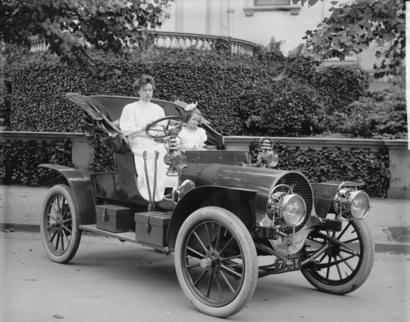
\includegraphics[width=\linewidth]{sample-franklin}
%   \caption{1907 Franklin Model D roadster. Photograph by Harris \&
%     Ewing, Inc. [Public domain], via Wikimedia
%     Commons. (\url{https://goo.gl/VLCRBB}).}
%   \Description{The 1907 Franklin Model D roadster.}
% \end{figure}

% Your figures should contain a caption which describes the figure to
% the reader. Figure captions go below the figure. Your figures should
% {\bfseries also} include a description suitable for screen readers, to
% assist the visually-challenged to better understand your work.

% Figure captions are placed {\itshape below} the figure.

% \subsection{The ``Teaser Figure''}

% A ``teaser figure'' is an image, or set of images in one figure, that
% are placed after all author and affiliation information, and before
% the body of the article, spanning the page. If you wish to have such a
% figure in your article, place the command immediately before the
% \verb|\maketitle| command:
% \begin{verbatim}
%   \begin{teaserfigure}
%     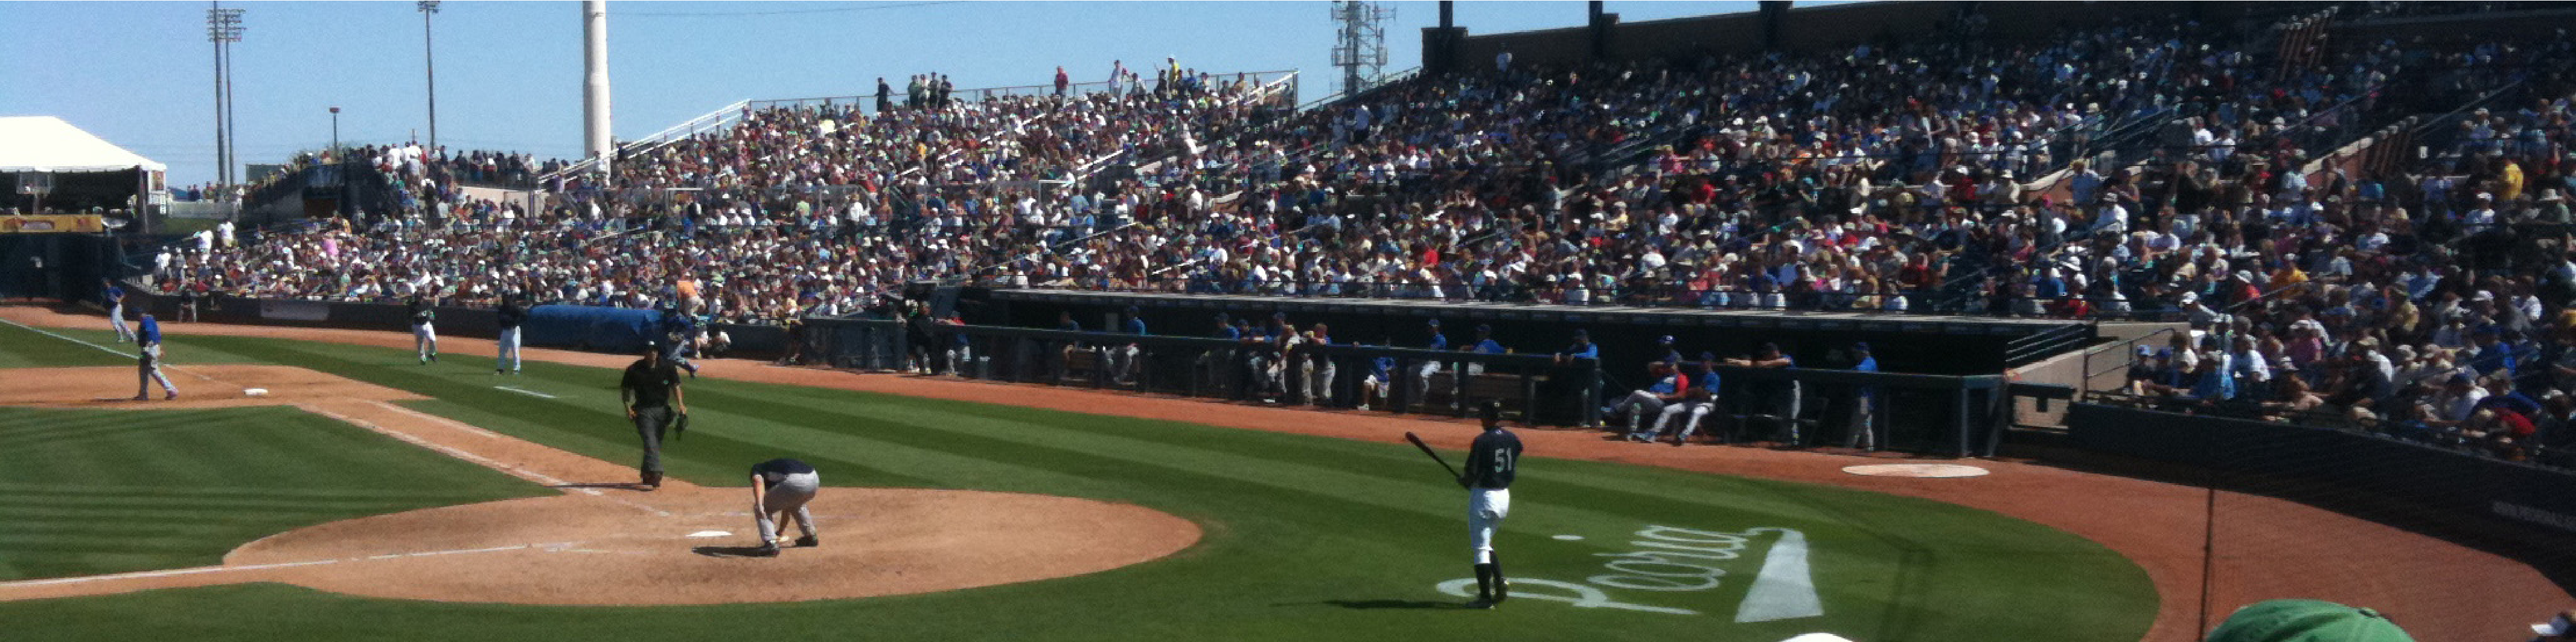
\includegraphics[width=\textwidth]{sampleteaser}
%     \caption{figure caption}
%     \Description{figure description}
%   \end{teaserfigure}
% \end{verbatim}

% \section{Citations and Bibliographies}

% The use of \BibTeX\ for the preparation and formatting of one's
% references is strongly recommended. Authors' names should be complete
% --- use full first names (``Donald E. Knuth'') not initials
% (``D. E. Knuth'') --- and the salient identifying features of a
% reference should be included: title, year, volume, number, pages,
% article DOI, etc.

% The bibliography is included in your source document with these two
% commands, placed just before the \verb|\end{document}| command:
% \begin{verbatim}
%   \bibliographystyle{ACM-Reference-Format}
%   \bibliography{bibfile}
% \end{verbatim}
% where ``\verb|bibfile|'' is the name, without the ``\verb|.bib|''
% suffix, of the \BibTeX\ file.

% Citations and references are numbered by default. A small number of
% ACM publications have citations and references formatted in the
% ``author year'' style; for these exceptions, please include this
% command in the {\bfseries preamble} (before
% ``\verb|\begin{document}|'') of your \LaTeX\ source:
% \begin{verbatim}
%   \citestyle{acmauthoryear}
% \end{verbatim}

%   Some examples.  A paginated journal article \cite{Abril07}, an
%   enumerated journal article \cite{Cohen07}, a reference to an entire
%   issue \cite{JCohen96}, a monograph (whole book) \cite{Kosiur01}, a
%   monograph/whole book in a series (see 2a in spec. document)
%   \cite{Harel79}, a divisible-book such as an anthology or compilation
%   \cite{Editor00} followed by the same example, however we only output
%   the series if the volume number is given \cite{Editor00a} (so
%   Editor00a's series should NOT be present since it has no vol. no.),
%   a chapter in a divisible book \cite{Spector90}, a chapter in a
%   divisible book in a series \cite{Douglass98}, a multi-volume work as
%   book \cite{Knuth97}, an article in a proceedings (of a conference,
%   symposium, workshop for example) (paginated proceedings article)
%   \cite{Andler79}, a proceedings article with all possible elements
%   \cite{Smith10}, an example of an enumerated proceedings article
%   \cite{VanGundy07}, an informally published work \cite{Harel78}, a
%   doctoral dissertation \cite{Clarkson85}, a master's thesis:
%   \cite{anisi03}, an online document / world wide web resource
%   \cite{Thornburg01, Ablamowicz07, Poker06}, a video game (Case 1)
%   \cite{Obama08} and (Case 2) \cite{Novak03} and \cite{Lee05} and
%   (Case 3) a patent \cite{JoeScientist001}, work accepted for
%   publication \cite{rous08}, 'YYYYb'-test for prolific author
%   \cite{SaeediMEJ10} and \cite{SaeediJETC10}. Other cites might
%   contain 'duplicate' DOI and URLs (some SIAM articles)
%   \cite{Kirschmer:2010:AEI:1958016.1958018}. Boris / Barbara Beeton:
%   multi-volume works as books \cite{MR781536} and \cite{MR781537}. A
%   couple of citations with DOIs:
%   \cite{2004:ITE:1009386.1010128,Kirschmer:2010:AEI:1958016.1958018}. Online
%   citations: \cite{TUGInstmem, Thornburg01, CTANacmart}.

% \section{Acknowledgments}

% Identification of funding sources and other support, and thanks to
% individuals and groups that assisted in the research and the
% preparation of the work should be included in an acknowledgment
% section, which is placed just before the reference section in your
% document.

% This section has a special environment:
% \begin{verbatim}
%   \begin{acks}
%   ...
%   \end{acks}
% \end{verbatim}
% so that the information contained therein can be more easily collected
% during the article metadata extraction phase, and to ensure
% consistency in the spelling of the section heading.

% Authors should not prepare this section as a numbered or unnumbered {\verb|\section|}; please use the ``{\verb|acks|}'' environment.

% \section{Appendices}

% If your work needs an appendix, add it before the
% ``\verb|\end{document}|'' command at the conclusion of your source
% document.

% Start the appendix with the ``\verb|appendix|'' command:
% \begin{verbatim}
%   \appendix
% \end{verbatim}
% and note that in the appendix, sections are lettered, not
% numbered. This document has two appendices, demonstrating the section
% and subsection identification method.

% \section{SIGCHI Extended Abstracts}

% The ``\verb|sigchi-a|'' template style (available only in \LaTeX\ and
% not in Word) produces a landscape-orientation formatted article, with
% a wide left margin. Three environments are available for use with the
% ``\verb|sigchi-a|'' template style, and produce formatted output in
% the margin:
% \begin{itemize}
% \item {\verb|sidebar|}:  Place formatted text in the margin.
% \item {\verb|marginfigure|}: Place a figure in the margin.
% \item {\verb|margintable|}: Place a table in the margin.
% \end{itemize}

%%
%% The acknowledgments section is defined using the "acks" environment
%% (and NOT an unnumbered section). This ensures the proper
%% identification of the section in the article metadata, and the
%% consistent spelling of the heading.
\begin{acks}
This work is partially supported by INCT-MACC, CNPq, CAPES and FAPERJ.
\end{acks}

%%
%% The next two lines define the bibliography style to be used, and
%% the bibliography file.
\bibliographystyle{ACM-Reference-Format}
\bibliography{mybib}

%%
%% If your work has an appendix, this is the place to put it.
% \appendix

% \section{Research Methods}

% \subsection{Part One}

% Lorem ipsum dolor sit amet, consectetur adipiscing elit. Morbi
% malesuada, quam in pulvinar varius, metus nunc fermentum urna, id
% sollicitudin purus odio sit amet enim. Aliquam ullamcorper eu ipsum
% vel mollis. Curabitur quis dictum nisl. Phasellus vel semper risus, et
% lacinia dolor. Integer ultricies commodo sem nec semper.

% \subsection{Part Two}

% Etiam commodo feugiat nisl pulvinar pellentesque. Etiam auctor sodales
% ligula, non varius nibh pulvinar semper. Suspendisse nec lectus non
% ipsum convallis congue hendrerit vitae sapien. Donec at laoreet
% eros. Vivamus non purus placerat, scelerisque diam eu, cursus
% ante. Etiam aliquam tortor auctor efficitur mattis.

% \section{Online Resources}

% Nam id fermentum dui. Suspendisse sagittis tortor a nulla mollis, in
% pulvinar ex pretium. Sed interdum orci quis metus euismod, et sagittis
% enim maximus. Vestibulum gravida massa ut felis suscipit
% congue. Quisque mattis elit a risus ultrices commodo venenatis eget
% dui. Etiam sagittis eleifend elementum.

% Nam interdum magna at lectus dignissim, ac dignissim lorem
% rhoncus. Maecenas eu arcu ac neque placerat aliquam. Nunc pulvinar
% massa et mattis lacinia.

\end{document}
\endinput
%%
%% End of file `sample-authordraft.tex'.
